% Feasible flow replacement used by the operating-profit ordering proof.
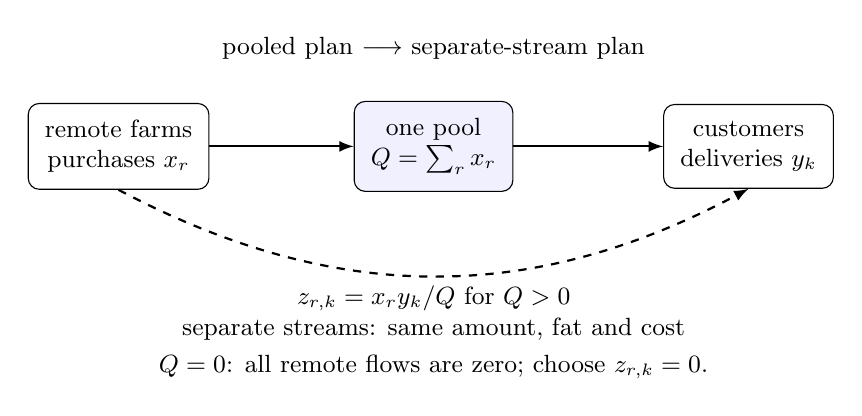
\begin{tikzpicture}[>=latex, every node/.style={font=\small},
 box/.style={draw,rounded corners,align=center,inner sep=6pt}]
\node[box] (remote) at (0,0) {remote farms\\purchases $x_r$};
\node[box,fill=blue!6] (pool) at (4,0) {one pool\\$Q=\sum_r x_r$};
\node[box] (cust) at (8,0) {customers\\deliveries $y_k$};
\draw[->,thick] (remote) -- (pool);
\draw[->,thick] (pool) -- (cust);
\draw[->,dashed,thick] (remote.south) to[bend right=28]
 node[below=0pt,align=center] {$z_{r,k}=x_r y_k/Q$ for $Q>0$\\separate streams: same amount, fat and cost} (cust.south);
\node[align=center] at (4,1.25) {pooled plan $\longrightarrow$ separate-stream plan};
\node[align=center] at (4,-2.8) {$Q=0$: all remote flows are zero; choose $z_{r,k}=0$.};
\end{tikzpicture}
